\section{Auswertung}
\label{sec:Auswertung}

\subsection{Kontrast}
\label{subsec:Kontrast}
Zu Beginn der Auswertung wurde der maximale Kontrast ermitttelt, der dann für die weitere Auswertung verwendet wurde.
Wie in \autoref{subsec:Kontrastbestimmmung} beschrieben, wurden die Messpunkte aufgenommen und mithilfe von \autoref{eqn:kontrast} wurde der Kontrast bestimmt.
Die Ergebnisse sind in \autoref{tab:Kontrast} zu finden.
Der maximale Kontrast mit $K = \num{0.97}$ wurde bei $\phi = \SI{135}{\degree}$ bestimmt.
Somit wurde der Polarisatiosfilter für die folgenden Messungen auf $\phi = \SI{135}{\degree}$ gestellt.

\noindent
Desweiteren wird mit den Messwerten eine Ausgleichsrechnung mit python durchgeführt.
Der Kontrast $K$ kann mit folgender Funktion beschrieben werden:
\begin{equation*}
  K = A \cdot | \cos(\Phi)\sin(\Phi) | \, .
\end{equation*}
Durch die Ausgleichsrechnung wird für 
\begin{equation*}
  A = 1,89 \pm 0,05
\end{equation*} 
ermittelt.
Die aufgenommenen Messwerte, sowie die Ausgleichsfunktion sind in \autoref{fig:Kontrast_Ausgleich} grafisch abgebildet.

\begin{figure}[H]
  \centering
  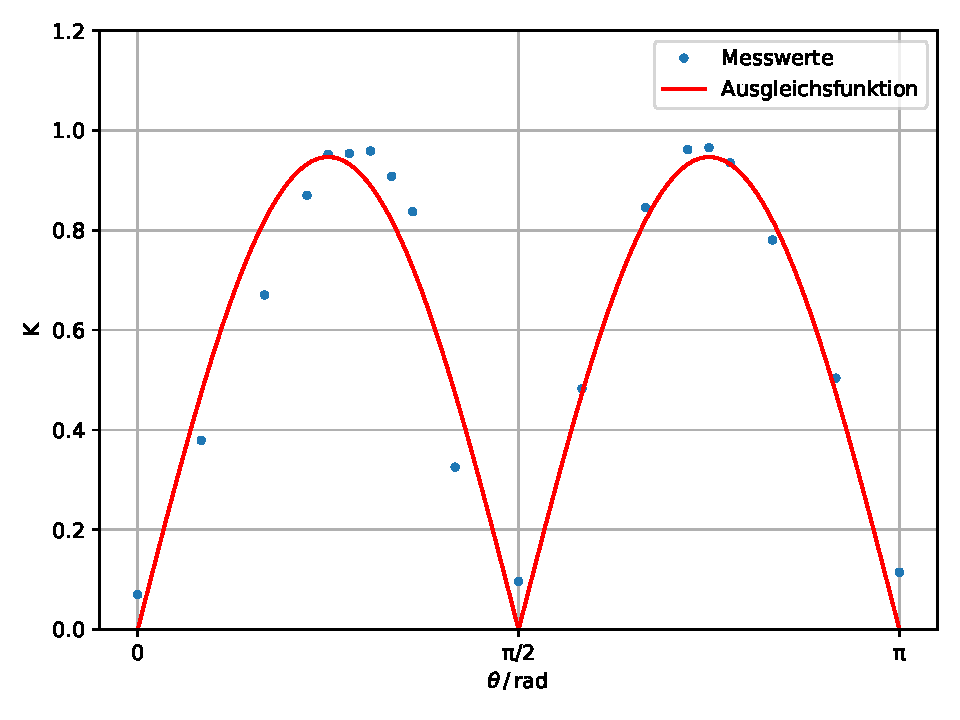
\includegraphics[width=\textwidth]{build/kontrast_ausgleich.pdf}
  \caption{Die aufgenommenen Messwerte zur Ermittlung des Kontrasts und die Ausgleichsrechnung.}
  \label{fig:Kontrast_Ausgleich}
\end{figure}

\begin{table}[H]
  \centering
  \caption{Aufgenommene Messwerte zur Kontrastmessung, sowie der jeweilige Kontrastwert.}
  \label{tab:Kontrast}
  \begin{tabular}{c c c c}
    \toprule
    $\Phi / \si{\degree} $ & $U_{\text{min}} / \si{\volt}$ & $U_{\text{max}} / \si{\volt}$ & $K$ \\
    \midrule
    0     &  0,86  &  0,99  & 0,07  \\
    15    &  0,36  &  0,80  & 0,38  \\
    30    &  0,14  &  0,71  & 0,67  \\
    40    &  0,05  &  0,72  & 0,87  \\
    45    &  0,02  &  0,82  & 0,95  \\
    50    &  0,02  &  0,85  & 0,95  \\
    55    &  0,02  &  0,96  & 0,96  \\
    60    &  0,05  &  1,04  & 0,91  \\
    65    &  0,10  &  1,13  & 0,84  \\
    75    &  0,58  &  1,14  & 0,33  \\
    90    &  0,84  &  1,02  & 0,10  \\
    105   &  0,60  &  1,72  & 0,48  \\
    120   &  0,22  &  2,63  & 0,85  \\
    130   &  0,06  &  3,08  & 0,96  \\
    135   &  0,05  &  2,85  & 0,97  \\
    140   &  0,10  &  3,00  & 0,94  \\
    150   &  0,32  &  2,60  & 0,78  \\
    165   &  0,62  &  1,88  & 0,50  \\
    180   &  0,77  &  0,97  & 0,11  \\
    \bottomrule
  \end{tabular}
\end{table}

\subsection{Brechungsindex von Glas}
\label{subsec:n_Glas}
Um den Brechungsindex von Glas zu bestimmen, wurde die Anzahl der Intensitätsminima $M$, wie in der \autoref{subsec:n_glas_Durchführung} beschrieben, aufgenommen.
Mithilfe der \autoref{eqn:n_Glas} wurde der Brechungsindex bestimmt.
Dabei beträgt die Dicke der Platten $D = \SI{1}{\milli\metre}$, die Wellenlänge des Lasers $\lambda_0 = \SI{632.990}{\nano\metre}$ und $\theta_0 = 10°$, da die beiden Platten jeweils um $\theta_0$ geneigt waren \cite{anleitung}.
Die aufgenommenen Messwerte sowie der jeweils ermittelte Brechungsindex sind in \autoref{tab:Glas} zu finden.
Im Mittel beträgt der ermittelte Brechungsindex für Glas 
\begin{equation*}
    n_\text{Glas} = 1,0001079364890089 \,.
\end{equation*}

\begin{table}[H]
  \centering
  \caption{Aufgenommene Messwerte zur Bestimmung des Brechungsindex von Glas, sowie der ermittelte Brechungsindex.}
  \label{tab:Glas}
  \begin{tabular}{c c c}
    \toprule
    Durchgang & M & $n_\text{Glas}$ \\
    \midrule
    1    &   30    &   1,00009496\\   
    2    &   35    &   1,00011079\\   
    3    &   36    &   1,00011395\\   
    4    &   36    &   1,00011395\\   
    5    &   35    &   1,00011079\\   
    6    &   35    &   1,00011079\\   
    7    &   35    &   1,00011079\\   
    8    &   36    &   1,00011395\\   
    9    &   31    &   1,00009812\\   
    10   &   32    &   1,00010129\\   
    \bottomrule
  \end{tabular}
\end{table}

\subsection{Brechungsindex von Luft}
\label{subsec:n_Luft}
Zur Bestimmung des Brechungsindex von Luft wurden die Messwerte, wie in \autoref{subsec:Durchführung_n_Luft} beschrieben, aufgenommen und mithilfe von \autoref{eqn:n_Luft} ermittelt.
Die Länge der Gaskammer beträgt $L = \SI[separate-uncertainty = true]{100(1)}{\milli\metre}$ \cite{anleitung} und die aufgenommene Temperatur $T = \SI{21.1}{\celsius}$.
Die aufgenommenen Messwerte sind in \autoref{tab:Luft} zu finden.
Der durchschnittliche Brechungsindex für jeden Durchgang ist in \autoref{tab:n_luft_mean} aufgelistet.
Für den durchschnittlichen Brechungsindex ohne Haube wurde
\begin{equation*}
  n_\text{Luft,ohne} = 1,0001703 \pm 0,0000017
\end{equation*}
und mit Haube 
\begin{equation*}
  n_\text{Luft,mit} =  1,0001622 \pm 0,0000016 \, .
\end{equation*}

\begin{table}[H]
  \centering
  \caption{Aufgenommene Messwerte zur Bestimmung des Brechungsindex von Luft.}
  \label{tab:Luft}
  \begin{tabular}{c c c c c}
    \toprule
    & \multicolumn{2}{c}{Durchgänge ohne Haube} & \multicolumn{2}{c}{Durchgänge mit Haube} \\
    \cmidrule(lr){2-3} \cmidrule(lr){4-5}
    $p / \si{\milli\bar}$ & 1 &2 &3 &4  \\
    \midrule
    50    &   4    &   5    &   2     &    2   \\
    100   &   6    &   7    &   4     &    4   \\
    150   &   8    &   10   &   7     &    10  \\
    200   &   10   &   122  &   9     &    12  \\
    250   &   12   &   14   &   11    &    14  \\
    300   &   14   &   16   &   13    &    21  \\
    350   &   17   &   18   &   15    &    23  \\
    400   &   20   &   20   &   17    &    25  \\
    450   &   23   &   22   &   19    &    27  \\
    500   &   25   &   24   &   21    &    29  \\
    550   &   28   &   26   &   24    &    31  \\
    600   &   32   &   29   &   26    &    34  \\
    650   &   36   &   31   &   28    &    36  \\
    700   &   39   &   33   &   30    &    38  \\
    750   &   42   &   35   &   32    &    40  \\
    800   &   44   &   37   &   34    &    42  \\
    850   &   47   &   39   &   36    &    44  \\
    900   &   50   &   41   &   38    &    46  \\
    950   &   54   &   43   &   41    &    48  \\
    1000  &   58   &   45   &   42    &    50  \\ 
    \bottomrule
  \end{tabular}
\end{table}

\begin{table}[H]
  \centering
  \caption{Der durchschnittliche Brechungsindex von Luft für jeden Durchgang. Durchgang 1 und 2 wurden ohne Haube durchgeführt, Durchgang 3 und 4 mit.}
  \label{tab:n_luft_mean}
  \begin{tabular}{c c}
    \toprule
    Durchgang & $n_\text{Glas}$ \\
    \midrule
    1    &  $1,0001801 \pm 0,0000018$ \\   
    2    &  $1,0001605 \pm 0,0000016$ \\   
    3    &  $1,0001823 \pm 0,0000018$ \\   
    4    &  $1,0001421 \pm 0,0000014$ \\   
    \bottomrule
  \end{tabular}
\end{table}

\subsubsection{Lorentz-Lorenz Gesetz}
Da der Brechungsindex von Gasen nach dem Lorentz-Lorenz Gesetz auch Druck und Temperatur abhängig ist, wird nach \autoref{eqn:Lorentz_Lorenz} eine Ausgleichsrechnung durchgeführt.
Die Ausgleichsfunktion hat dabei die Form
\begin{equation*}
  n = \frac{a}{TR} \cdot p + b \, .
\end{equation*}
Nach einer Temperaturmessung ergab sich für $T = \SI{21.1}{\celsius} = \SI{294.25}{\kelvin}$, $R$ beschreibt die universale Gaskonstante.
Die Ausgleichsrechnung wird für alle vier Durchgänge gemacht.
Für die Variablen $a$ und $b$ ergibt sich somit folgende Werte:
\begin{table}[H]
  \centering
  \caption{Die Ergebnisse der Ausgleichsrechnung für die Variablen $a$ und $b$ je Durchgang. Durchgang 1 und 2 wurden ohne Haube durchgeführt, Durchgang 3 und 4 mit.}
   \begin{tabular}{c c c}
    \toprule
    Messung & $a / \si{\cubic\metre\per\mole}$ & $b$ \\
    \midrule
    1    &  $0,00089 \pm 1,70357$ & $0,99998 \pm 4,17067$ \\   
    2    &  $0,00065 \pm 3,68946$ & $1,00002 \pm 9,03250$ \\   
    3    &  $0,00076 \pm 2,42896$ & $1,00002 \pm 5,94660$ \\   
    4    &  $0,00066 \pm 4,15068$ & $1,00000 \pm 1,01617$ \\
    \bottomrule
  \end{tabular}
\end{table}
\noindent
Die aus den Messwerten berechneten Brechungsindizes und die daraus ermittelten Ausgleichsgraden sind in \autoref{fig:lorentz_lorenz} zu finden.

\noindent
Im Durchschnitt haben die Variablen folgenden Wert:
\begin{align*}
  a = 0,000740 \pm 0,000008 \, \si{\cubic\metre\per\mole}& &b = 1,0000075 \pm 0,0000018
\end{align*}
Nach dem Lorentz-Lorenz Gesetz beträgt der Brechungsindex von Luft mit diesen Werten und bei Normatmosphäre 
\begin{equation*}
  n = 1,0000078 \pm 0,0000018 \, .
\end{equation*}
Dabei ist $T = \SI{15}{\celsius} = \SI{288.15}{\kelvin}$ und $p = \SI{1013}{\hecto\pascal}$.

\begin{figure}[H]
  \centering
  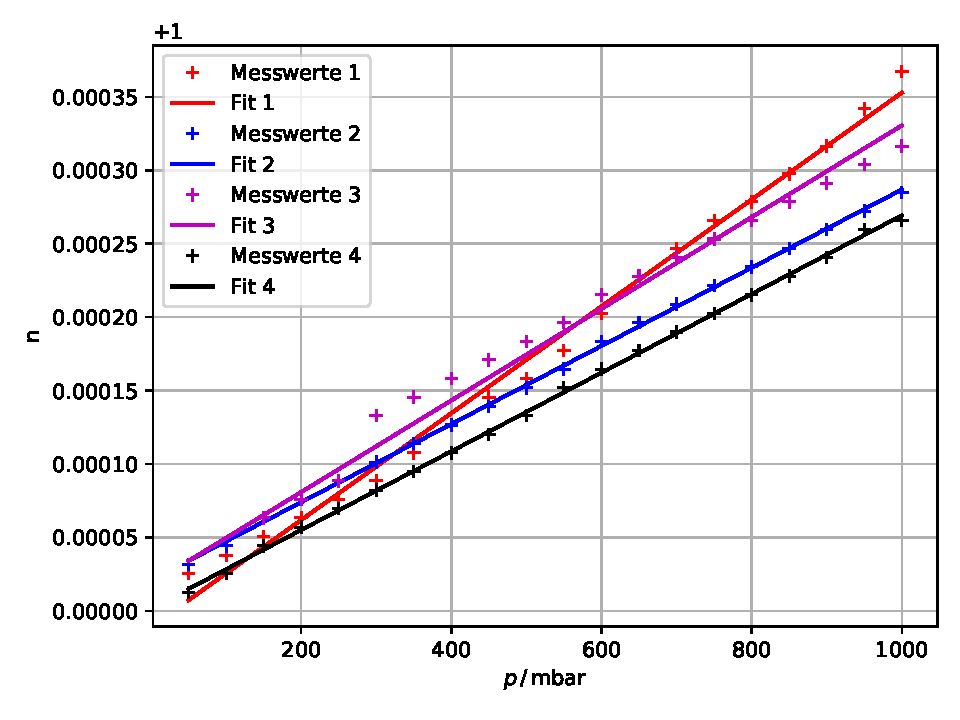
\includegraphics[width=\textwidth]{build/lorentz_lorenz.pdf}
  \caption{Die aus den aufgenommenen Messwerten bestimmten Brechungsindizes $n$ für Luft und die Ausgleichsgraden.
  Messung 1 und 2 wurden ohne Haube durchgeführt, Messung 3 und 4 mit.}
  \label{fig:lorentz_lorenz}
\end{figure}

